
%(BEGIN_QUESTION)
% Copyright 2015, Tony R. Kuphaldt, released under the Creative Commons Attribution License (v 1.0)
% This means you may do almost anything with this work of mine, so long as you give me proper credit

Suppose a control valve is used to throttle liquid into a reservoir which then gravity-drains to a process.  A level-control system (not shown) commands the control valve as needed to maintain a constant liquid level in the reservoir, over a typical flow range of 0 to 100 gallons per minute:

$$\includegraphics[width=15.5cm]{i01180x02.eps}$$

Based on the information shown in the simple PFD and pump curve, determine whether a control valve with linear characteristics will actually behave in a linear manner (i.e. have linear {\it installed} characteristics) in this process.  Explain your reasoning in detail.

\vskip 10pt

Next, determine the same for the following process, where the control valve throttles liquid through a spray nozzle over the same typical flow range of 0 to 100 GPM:

$$\includegraphics[width=15.5cm]{i01180x01.eps}$$

\vskip 20pt \vbox{\hrule \hbox{\strut \vrule{} {\bf Suggestions for Socratic discussion} \vrule} \hrule}

\begin{itemize}
\item{} Explain in a general sense where and why we may need a ``characterized'' control valve to achieve linear flow control in any given process.
\item{} Will control valves of the same $C_v$ rating work equally well in both scenarios?  Explain why or why not.  If different $C_v$ ratings are necessary, which scenario demands a control valve with a larger $C_v$?
\item{} It is generally bad practice to ``dead-head'' a centrifugal pump (i.e. to completely block its discharge line while running, as this control valve will do when shut).  Identify multiple ways to address this problem, so that the pump can never ``dead-head'' no matter what position the control valve is placed in.
\end{itemize}

\underbar{file i01180}
%(END_QUESTION)





%(BEGIN_ANSWER)

{\it Hint: does the pressure drop across the control valve vary substantially with flow?}
 
%(END_ANSWER)





%(BEGIN_NOTES)

The first process example (flowing into an open reservoir) will exhibit linear installed characteristics, because the pressure drop across the control valve will be nearly constant over the entire range of flow (0-100 GPM).  The pump curve shows discharge pressure to remain fairly flat (between about 70 to 77 PSI) over the expected flow range, and since the vertical head pressure (25 feet at a specific gravity of 0.85) is constant and the pipe discharge pressure is 0 (atmospheric) this means the control valve will see a relatively constant pressure drop:

$$\Delta P = 70 - \left(25 \hbox{ ft liquid} \over 1 \right)  \left(12 \hbox{ in} \over 1 \hbox{ ft}\right)  \left(1 \hbox{ PSI} \over 27.68 \hbox{ "WC}\right)  \left(0.85 \hbox{ "WC} \over 1 \hbox{ " liquid}\right) = 60.79 \hbox{ PSID minimum}$$

$$\Delta P = 77 - \left(25 \hbox{ ft liquid} \over 1 \right)  \left(12 \hbox{ in} \over 1 \hbox{ ft}\right)  \left(1 \hbox{ PSI} \over 27.68 \hbox{ "WC}\right)  \left(0.85 \hbox{ "WC} \over 1 \hbox{ " liquid}\right) = 67.79 \hbox{ PSID maximum}$$

A variation of 7 PSI is just a little more than 10\% of the baseline pressure drop across the valve.  Plotting this ``load line'' on top of a set of characteristic curves for an inherently linear valve, we see a set of intersections that are very nearly equally-spaced:

$$\includegraphics[width=15.5cm]{i01180x03.eps}$$

\vskip 10pt

\filbreak

In the second process example, however, the inclusion of a spray nozzle into the piping introduces a variable pressure drop of 0 to 25 PSID over the same flow range.  This means the valve's pressure drop will be 25 PSID less at full flow (100 GPM) while remaining the same as before at zero flow.  This larger, flow-dependent variation in available pressure will distort the control valve's installed characteristics, necessitating equal-percentage trim rather than (inherently) linear trim.

This larger variation creates a load line with a sharper curve, and consequently a set of intersections that are {\it not} equally-spaced:

$$\includegraphics[width=15.5cm]{i01180x04.eps}$$

Incidentally, this set of curves assumes the use of a larger control valve, in order to achieve the same maximum flow rate with less available pressure.

%INDEX% Final Control Elements, pump: pressure/flow curve
%INDEX% Final Control Elements, valve: characterization

%(END_NOTES)


